\documentclass{beamer}
%
% Choose how your presentation looks.
%
% For more themes, color themes and font themes, see:
% http://deic.uab.es/~iblanes/beamer_gallery/index_by_theme.html
%
\mode<presentation>
{
  \usetheme{Antibes}      % or try Darmstadt, Madrid, Warsaw, ...
  \usecolortheme{default} % or try albatross, beaver, crane, ...
  \usefonttheme{default}  % or try serif, structurebold, ...
  \setbeamertemplate{navigation symbols}{}
  \setbeamertemplate{caption}[numbered]
} 

\usepackage[english]{babel}
\usepackage[utf8x]{inputenc}
\usepackage{adjustbox}
\usepackage{ragged2e}
\graphicspath{ {./img/} }



\title[Investigating the Validity of Ground Truth in Code Reviewer Recommendation Studies]{Investigating the Validity of Ground Truth in Code Reviewer Recommendation Studies}
\author{Emre Dogan}
\institute{Bilkent University}
\date{June 17, 2019}

\begin{document}

\begin{frame}
  \titlepage
\end{frame}

% Outline
\begin{frame}{Outline}
  \tableofcontents
\end{frame}
%
%


\section{Introduction}

\begin{frame}{Introduction}

\begin{itemize}
  \item \textbf{Code Review:} An inspection of a code change by an independent third-party
developer in order to identify and fix defects before an integration to
improve software quality\cite{whoshould}.
  \item It is a challenging task to find the ideal reviewer for a changeset.
  \item There are several studies to recommend the ideal reviewer for a changeset:
  \begin{itemize}
      \item Heuristic Based  Approaches
      \item Machine Learning Approaches
      \item Graph Based Approaches
      \item Hybrid Approaches
  \end{itemize}
\end{itemize}

\vskip 1cm
\end{frame}
%
%
\section{Code Review Process}
\begin{frame}{Code Review}
    % Commands to include a figure:
    \begin{figure}
    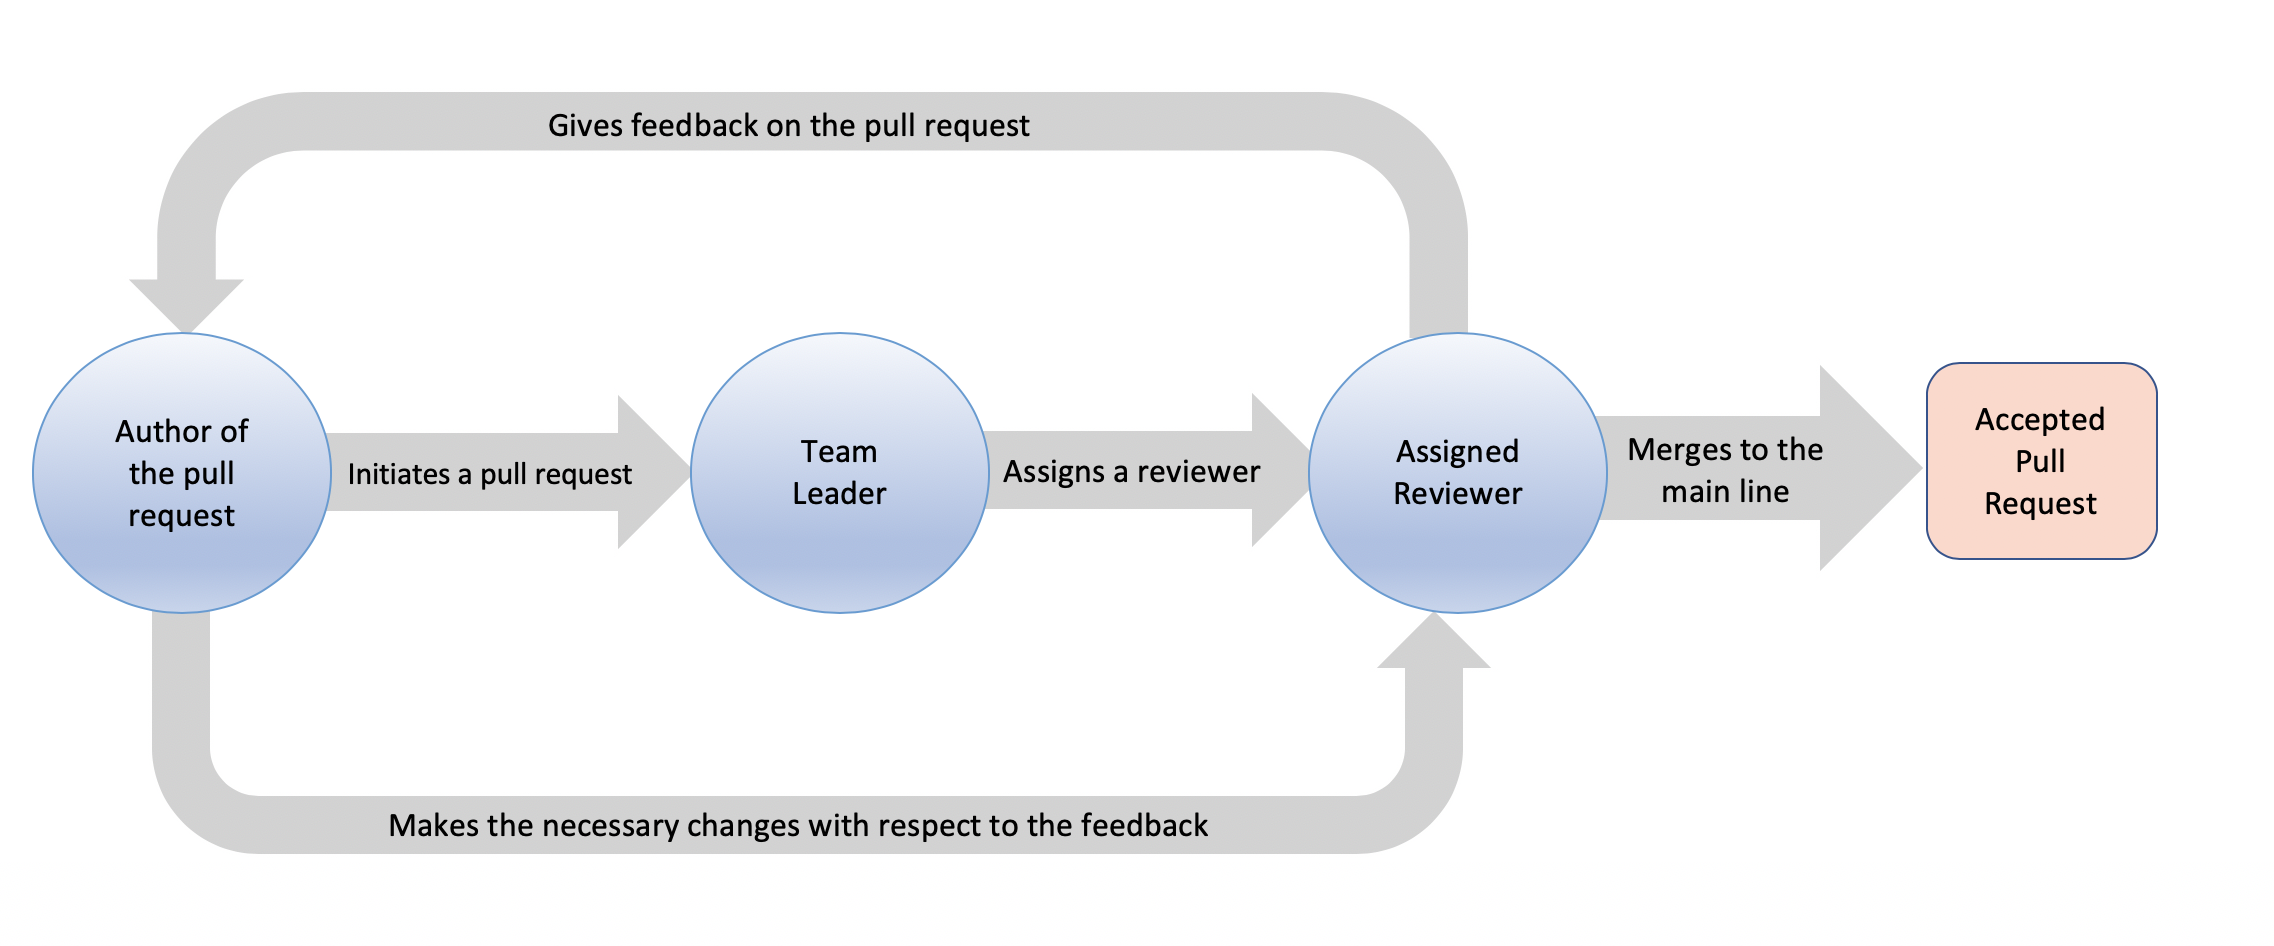
\includegraphics[width=\textwidth]{review.png}
    \caption{\label{fig:your-figure}A typical code review scenario in real life.}
    \end{figure}
\end{frame}

%
%
\section{Ground Truth}
\begin{frame}{Ground Truth}
    % Commands to include a figure:
    \begin{block}{Definition}
    \textbf{Ground Truth:} Ideal output label of an algorithm. 
    \end{block}

    \begin{block}{Ground Truth in Software Engineering}
    The more human aspects involved, the more tendency to the ground truth problems.  
    \end{block}
    
    \begin{block}{Ground Truth in Code Reviewer Recommendation Process}
    \begin{itemize}
        \item Recommendation studies rely on the real-life reviewer assignments.
        \item These studies assume that these assignments are ideal. 
        \item Studies in real-life projects (OSS or proprietary) show that code reviewers are not assigned with the aim of finding the ideal one.
    \end{itemize}
    \end{block}
\end{frame}
%
%
\section{Example Scenario}
\begin{frame}{Example Scenario}
    % Commands to include a figure:
    \begin{figure}
    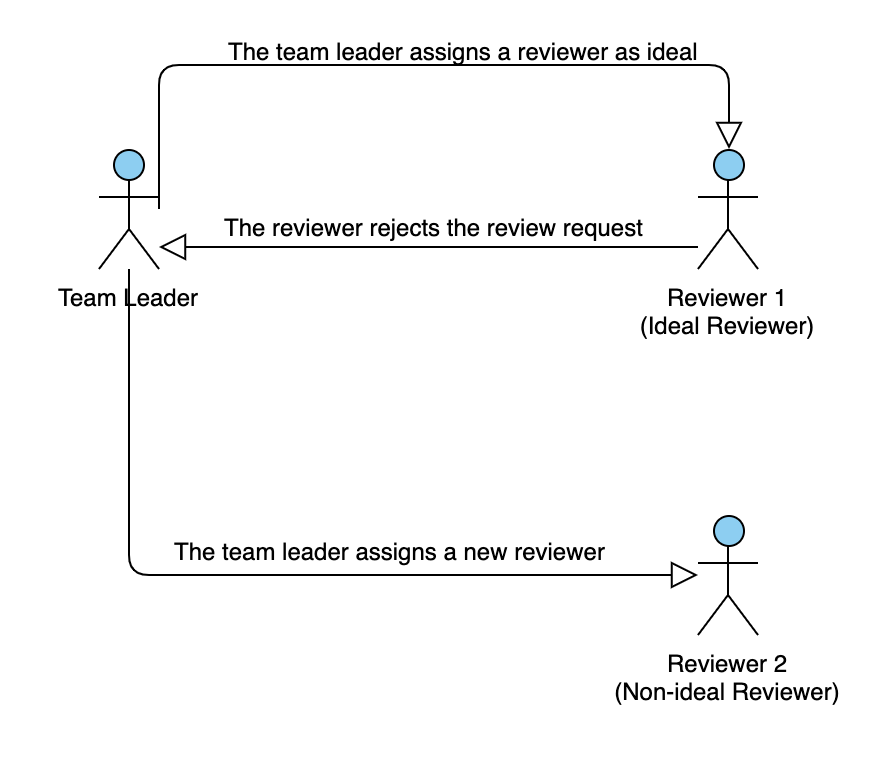
\includegraphics[width=8cm]{img/scenario.png}
    \caption{\label{fig:your-figure}Problematic reviewer assignment scenario}
    \end{figure}
\end{frame}

%
%
\section{Problem Definition}
\begin{frame}{Problem Definition}
    % Commands to include a figure:
    \begin{figure}
    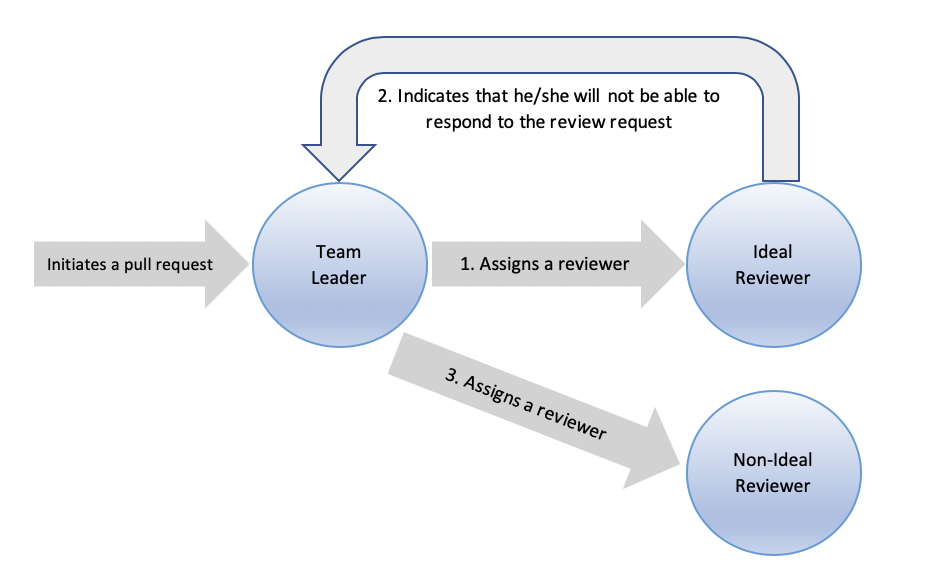
\includegraphics[width=10cm]{ideal-review.png}
    \caption{\label{fig:your-figure}Ideal Reviewer Selection Problem.}
    \end{figure}
\end{frame}

\begin{frame}{Problem Definition-II}
    % Commands to include a figure:
    \begin{figure}
    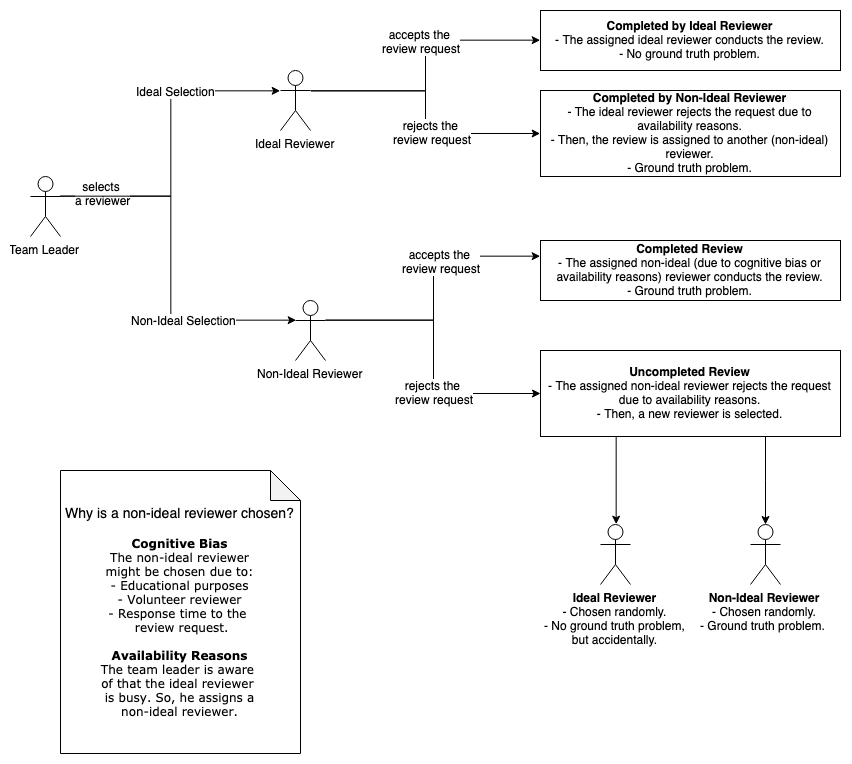
\includegraphics[width=8cm]{new-figure.png}
    \caption{\label{fig:your-figure}Ideal Reviewer Selection Problem.}
    \end{figure}
\end{frame}
%
\begin{frame}{A Set of Real-Life Scenarios}
\begin{table}[h!]
\resizebox{\textwidth}{!}{%
\begin{tabular}{l|l|l|l|l|l|l|l}
Pull Request & Actual Reviewer & Ideal Reviewer & \begin{tabular}[c]{@{}c@{}}Recommended \\ Reviewer\end{tabular} & Case          & \begin{tabular}[c]{@{}c@{}}Correctness of Algorithm \\ w.r.t. Actual Reviewer\end{tabular} & \begin{tabular}[c]{@{}c@{}}Correctness of Algorithm \\ w.r.t. Ideal Reviewer\end{tabular} & \begin{tabular}[c]{@{}c@{}}Ground Truth \\ Validity\end{tabular} \\ \hline
1            & John            & John           & John                 & r=a  and  a=i & \checkmark                                                                                          & \checkmark                                                                                         & Yes                                                              \\ \hline
2            & John            & Mary           & John                 & r=a  and  a≠i & \checkmark                                                                                          & X                                                                                         & No                                                               \\ \hline
3            & John            & Mary           & Mary                 & r≠a  and  a≠i & X                                                                                          & \checkmark                                                                                         & No                                                               \\ \hline
4            & John            & John           & Mary                 & r≠a  and  a=i & X                                                                                          & X                                                                                         & Yes                                                              \\ \hline
5            & John            & Mary           & James                & r≠a  and  a≠i & X                                                                                          & X                                                                                         & No
\end{tabular}
}
\caption{\label{tab:widgets} Real-life scenarios to illustrate the ground truth problem.}
\scriptsize\textit{r: recommended reviewer, a: actual reviewer, i: ideal reviewer}

\end{table}

\begin{block}{Notice}
Pull Requests 2, 3 and 5 have a problematic ground truth definition.
\end{block}

% Commands to include a figure:
%\begin{figure}
%\includegraphics[width=\textwidth]{your-figure's-file-name}
%\caption{\label{fig:your-figure}Caption goes here.}
%\end{figure}

\end{frame}
%


\section{Review Selection}
\subsection{Review Selection in Real Life}
    \begin{frame}{How Reviewers are Selected in Real Life}
\begin{table}
\centering
\begin{tabular}{c|c}
Related Studies & Considered Method \\\hline
\cite{kovalenko2018does,ruangwan2019impact,kononenko2015investigating} & Reviewer experience \\
\cite{kovalenko2018does,macleod2017code} & Code familiarity  \\
\cite{ruangwan2019impact,kononenko2015investigating} & Patch characteristics \\
\textbf{\cite{kovalenko2018does,macleod2017code}} & \textbf{Volunteer for review} \\
\textbf{\cite{kovalenko2018does,ruangwan2019impact}} & \textbf{Workload} \\
\textbf{\cite{kovalenko2018does}} & \textbf{Physical Proximity} \\
\textbf{\cite{kovalenko2018does}} & \textbf{Availability}  \\
\textbf{\cite{kovalenko2018does}} & \textbf{Response time to review requests} \\
\textbf{\cite{macleod2017code}} & \textbf{Training the new hires} 

\end{tabular}
\caption{\label{tab:widgets} Real-life factors affecting reviewer selection.}
\end{table}

\end{frame}
%
%
%

\subsection{Review Selection in Recommendation Models}
    \begin{frame}{Recommendation Models}
        
        \begin{table}[]
\centering
\adjustbox{max height=\dimexpr\textheight-5.5cm\relax,
           max width=\textwidth}{

        \centering
        \begin{tabular}{c}
        
        \textbf{APPLIED METHOD} \\ \hline
        Bayesian Network \\ \hline
        Change History of Source Code Lines \\ \hline
        Decision Tree \\ \hline
        Expertise in Related Technologies \\ \hline
        Genetic Algorithm \\ \hline
        Information Retrieval \\ \hline
        K-nearest neighbors (KNN) \\ \hline
        Latent Dirichlet Allocation \\ \hline
        Latent Factor \& Neighborhood \\ \hline
        Path Similarity \\ \hline
        Previous Review Success \\ \hline
        Random Forest \\ \hline
        Social Network Analysis \\ \hline
        Support Vector Machines \\ \hline
        Text Similarity of PR Requests \\ 
        \end{tabular}}
        \caption{Automated Reviewer Recommendation Methods}
        \label{tab:my-table}
        \end{table}



    \end{frame}

\section{Quantitative Evidence for the Ground Truth Problem}
    
    \begin{frame}{Comparison of Real Life and Recommendation Studies}
        \begin{block}{Hypothesis}
            \centering
            Reviewer selection process takes place differently in real life and recommendation models. 
        \end{block}
    \end{frame}    
    
    \begin{frame}{Quantitative Evidence}
        \begin{table}[]
        \centering
        \adjustbox{max height=\dimexpr\textheight-5.5cm\relax,
           max width=\textwidth}{
        \begin{tabular}{c|c|c|c}
        \textbf{Project Name} & \textbf{\begin{tabular}[c]{@{}c@{}}Total Number \\ of Pull Requests\end{tabular}} & \textbf{\begin{tabular}[c]{@{}c@{}}Number of PRs \\ with at least one \\ non-responsive reviewer\end{tabular}} & \textbf{\begin{tabular}[c]{@{}c@{}}The ratio of PRs \\ having at least one \\ non-responsive reviewer\end{tabular}} \\
        \hline
        Android & 36,771 & 24,367 & 66\% \\
        \hline
        LibreOffice & 18,716 & 3,039 & 16\% \\
        \hline
        Open Stack & 108,788 & 24,589 & 23\% \\
        \hline
        Qt & 65,815 & 30,630 & 47\% \\
        \hline
        TOTAL & 230,090 & 82,625 & 36\%
        \end{tabular}}
        \caption{PR Analysis of 4 Large OSS Projects \cite{ruangwan2019impact}.}
        \label{tab:my-table}
        \end{table}
    \end{frame}

\section{Solution Alternatives}
    \begin{frame}{Solution Alternatives}
    \begin{itemize}
        \item Expensive Setup in Real Life
        \item Forward-Looking Mining
    \end{itemize}
    \end{frame}


    \begin{frame}{Expensive Setup in Real Life}
        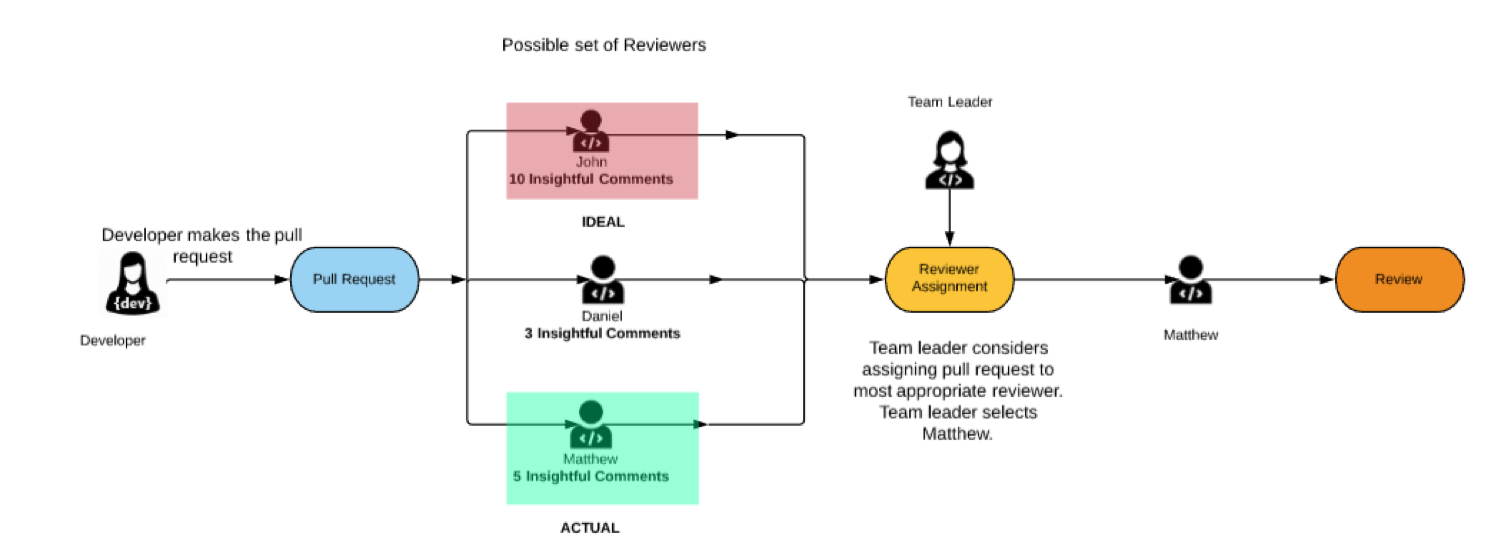
\includegraphics[height=4.4cm]{sol1}

    \end{frame}
    \begin{frame}{Expensive Setup in Real Life}
    i. To fix an issue, developer implements a solution and
    commits this solution as a pull request.
    
    ii. Team leader assigns every possible reviewer in the team
    as a single reviewer to the pull request.
    
    iii. Each reviewer reviews the request and provides
    comments.
    
    iv. Team leader or the developer selects the ideal review and
    reviewer based on metrics (i.e. providing insightful
    comments in the shortest time possible) among the
    reviewers and reviews. 

    \end{frame}

    \begin{frame}{Forward-Looking Mining}
        \begin{columns}
        \column{0.4\textwidth}
        \centering 
        - If a bug is reopened, it is a potential indicator that the assigned
        reviewer was not the ideal reviewer for that pull request. 
        
        - Deleting these instances will increase the validity of the dataset.
        \column{0.55\textwidth}
        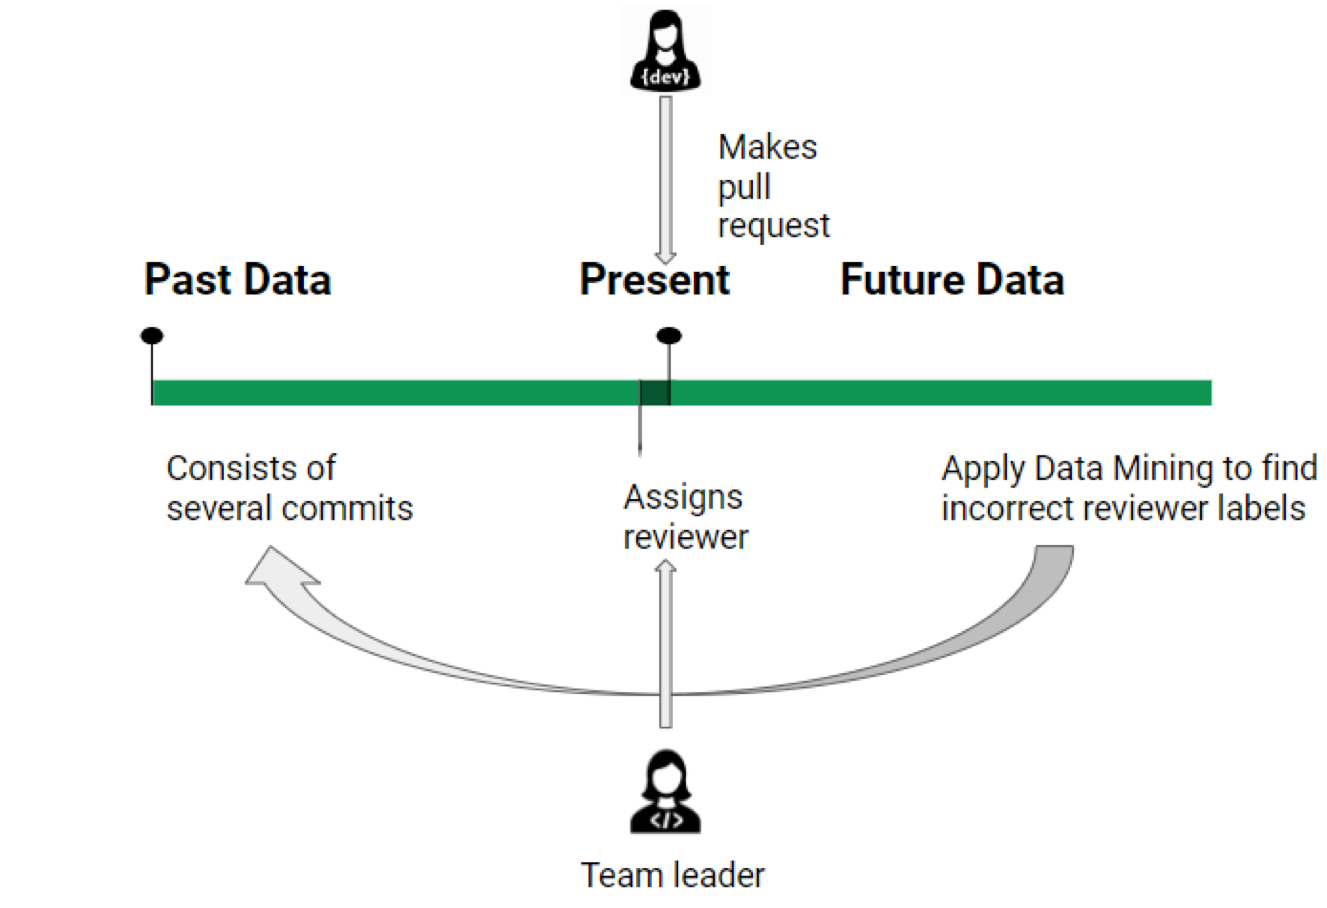
\includegraphics[height=4.8cm]{sol2}
        \end{columns}

    \end{frame}

\section{References}
\begin{frame}{References}

 \bibliographystyle{ieeetr}
 \tiny\bibliography{bib.bib}
\end{frame}

\end{document}

%\begin{block}{Examples}
%Some examples of commonly used commands and features are included, to help you get started.
%\end{block}